\begin{figure}[h]
  \centering
    \begin{tikzpicture}[inner sep=0pt, outer sep=0pt]
      \node[anchor=west] (A) at (0,0)
        {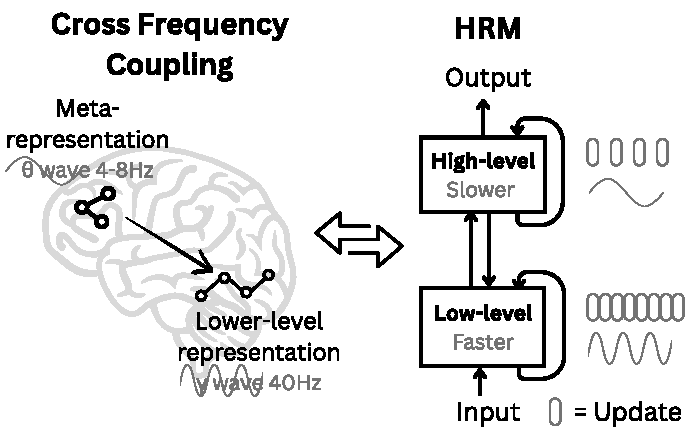
\includegraphics[width=0.35\linewidth]{figures/main_diagram/H-main-figure.pdf}};
      \node[anchor=east, xshift=0.1in] (B) at (\linewidth,0)
        {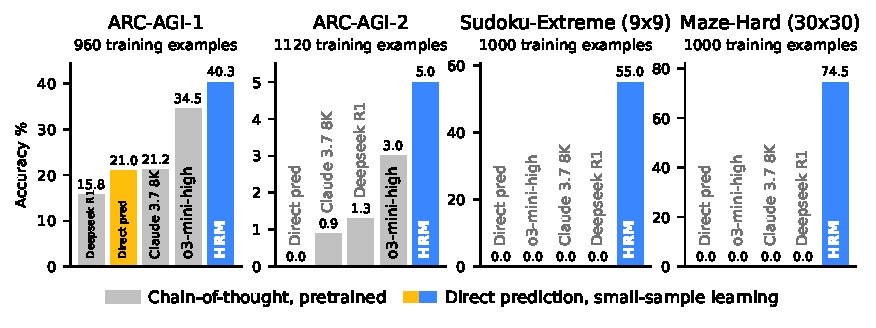
\includegraphics[width=0.65\linewidth]{figures/benchmark_bars/benchmark_bars.pdf}};
    \end{tikzpicture}
  \vspace*{-0.5ex}%
  \caption{\textbf{Left:} HRM is inspired by hierarchical processing and temporal separation in the brain. It has two recurrent networks operating at different timescales to collaboratively solve tasks. \textbf{Right:} With only about 1000 training examples, the HRM (\textasciitilde27M parameters) surpasses state-of-the-art CoT models on inductive benchmarks (ARC-AGI) and challenging symbolic tree-search puzzles (\textit{Sudoku-Extreme}, \textit{Maze-Hard}) where CoT models failed completely. The HRM was randomly initialized, and it solved the tasks directly from inputs without chain of thoughts.}
  \label{fig:benchmark_bars}
  \vspace*{-1ex}%
\end{figure}